% answers.tex —— 1977 年·安徽卷（文科） · 参考答案与详细解析片段
% 由 tools/generate_projects.py 依来源总账自 1977/1977_数学真题_安徽文_试题.md + 1977/1977_数学真题_安徽文_解析正文.md + 1977/1977_数学真题_安徽文_答案要点.md 生成，勿手改（改源 MD 后重跑）


\begin{gktip}
固定源 PDF 第 4—10 页附官方《解答和评分标准》（书籍页码 29—35「题解」）。下文逐题对照源解答重新计算关键结论，不照抄解答原文；源解答对第 1(4)、6、8 题另给出两到四种方法，本文各取一条主推路线。原卷函数记号 tg、大写 Cos 在本文件按现代记号展开（tan、cos）。
\end{gktip}

\begin{answer}
\gksolhead{1}{}

\textbf{题目}（本题25分，每小题5分）：

计算

（1） $5\frac{1}{2}\times\left(-\dfrac{6}{11}\right)+0.25-(-2)^3\div\left(-2\frac{2}{3}\right)^2$；

（2） $\sqrt{14\times24\times39\times91}+4\sqrt{27}\times(-\sqrt3)$；

（3） $\left(-2\frac{3}{5}\right)^0+4^{-2}\times\left(2\frac{1}{4}\right)^{-\frac{1}{2}}-(0.01)^{0.5}$；

（4） $\dfrac{2\lg2+\lg3}{2+\lg0.36+\dfrac{2}{3}\lg8}$；

（5） $\dfrac{\operatorname{tg}(-120^\circ)\cdot\operatorname{Cos}(-240^\circ)\cdot\operatorname{Cos}480^\circ}{\operatorname{tg}(-60^\circ)\cdot\sin(-1050^\circ)}$。

\Needspace{4\baselineskip}
\textbf{解析}

\gksubpart{（1）}

\nopagebreak[4]
\[
5\frac{1}{2}\times\left(-\frac{6}{11}\right)+\frac{1}{4}-(-8)\div\left(-\frac{8}{3}\right)^2
=-3+\frac{1}{4}-(-8)\times\frac{9}{64}
=-3+\frac{1}{4}+\frac{9}{8}=-\frac{13}{8}=-1\frac{5}{8}.
\]

\gksubpart{（2）}

\nopagebreak[4]
\[
\sqrt{14\times24\times39\times91}
=\sqrt{(2\times7)\times(2^3\times3)\times(3\times13)\times(7\times13)}
=\sqrt{2^4\cdot3^2\cdot7^2\cdot13^2}=2^2\times3\times7\times13=1092,
\]

\nopagebreak[4]
\[
4\sqrt{27}\times(-\sqrt3)=4\times3\sqrt3\times(-\sqrt3)=-36.
\]

故原式 $=1092-36=1056$。

\gksubpart{（3）}

\nopagebreak[4]
\[
\left(-2\frac{3}{5}\right)^0+4^{-2}\times\left(2\frac{1}{4}\right)^{-\frac{1}{2}}-(0.01)^{0.5}
=1+\frac{1}{16}\times\left(\frac{4}{9}\right)^{\frac{1}{2}}-0.1
=1+\frac{1}{16}\times\frac{2}{3}-\frac{1}{10}
=1+\frac{1}{24}-\frac{1}{10}=\frac{113}{120}.
\]

\gksubpart{（4）}

\Needspace{5\baselineskip}
分子 $=2\lg2+\lg3=\lg(2^2\times3)=\lg12$。分母中

\nopagebreak[4]
\[
\lg0.36=\lg\frac{36}{100}=\lg4+\lg9-2=2\lg2+2\lg3-2,
\qquad
\frac{2}{3}\lg8=\frac{2}{3}\times3\lg2=2\lg2,
\]

\Needspace{5\baselineskip}
故分母 $=2+(2\lg2+2\lg3-2)+2\lg2=4\lg2+2\lg3=2(2\lg2+\lg3)$，原式

\nopagebreak[4]
\[
=\frac{2\lg2+\lg3}{2(2\lg2+\lg3)}=\frac{1}{2}.
\]

\gksubpart{（5）}

\Needspace{5\baselineskip}
用诱导公式与周期性化简各因子：

\nopagebreak[4]
\[
\operatorname{tg}(-120^\circ)=\operatorname{tg}60^\circ=\sqrt3,
\qquad
\cos(-240^\circ)=\cos240^\circ=-\frac{1}{2},
\qquad
\cos480^\circ=\cos120^\circ=-\frac{1}{2},
\]

\nopagebreak[4]
\[
\operatorname{tg}(-60^\circ)=-\sqrt3,
\qquad
\sin(-1050^\circ)=\sin(-1050^\circ+3\times360^\circ)=\sin30^\circ=\frac{1}{2}.
\]

\Needspace{5\baselineskip}
于是

\nopagebreak[4]
\[
\text{\text{原式}}=\frac{\sqrt3\times\left(-\frac{1}{2}\right)\times\left(-\frac{1}{2}\right)}{(-\sqrt3)\times\frac{1}{2}}
=\frac{\frac{\sqrt3}{4}}{-\frac{\sqrt3}{2}}=-\frac{1}{2}.
\]

\gkanswer{答案（1）：$-1\frac{5}{8}$。}

\gkanswer{答案（2）：$1056$。}

\gkanswer{答案（3）：$\dfrac{113}{120}$。}

\gkanswer{答案（4）：$\dfrac{1}{2}$。}

\gkanswer{答案（5）：$-\dfrac{1}{2}$。}

\end{answer}
\begin{answer}
\gksolhead{2}{}

\textbf{题目}（本题满分10分，每小题5分）：

化简；

（1） $\left(3\sqrt[3]{a^2}\cdot\sqrt{b}\right)\cdot\left(-6\sqrt{a}\cdot\sqrt[3]{b}\right)\div\left(-2\sqrt[6]{a}\cdot\sqrt[6]{b^5}\right)$；

（2） $\sqrt{(\lg x)^2-2\lg x+1}$。

\Needspace{4\baselineskip}
\textbf{解析}

\gksubpart{（1）}

\Needspace{5\baselineskip}
按指数法则合并系数与各字母指数：

\nopagebreak[4]
\[
\frac{3\times(-6)}{-2}\,a^{\frac{2}{3}+\frac{1}{2}-\frac{1}{6}}\,b^{\frac{1}{2}+\frac{1}{3}-\frac{5}{6}}
=9\,a^{1}\,b^{0}=9a.
\]

（在各根式有意义的 $a\ge0$、$b\ge0$ 范围内化简。）

\gksubpart{（2）}

\Needspace{5\baselineskip}
被开方式是完全平方，在定义域 $x>0$ 内：

\nopagebreak[4]
\[
\sqrt{(\lg x)^2-2\lg x+1}=\sqrt{(\lg x-1)^2}=|\lg x-1|
=\begin{cases}
\lg x-1,&x\ge10,\\
1-\lg x,&0<x<10.
\end{cases}
\]

\gkanswer{答案（1）：$9a$。}

\gkanswer{答案（2）：$\sqrt{(\lg x-1)^2}=|\lg x-1|=\begin{cases}\lg x-1,&x\ge10,\\[2pt]1-\lg x,&0<x<10.\end{cases}$。}

\end{answer}
\begin{answer}
\gksolhead{3}{}

\textbf{题目}（满分5分）：

\Needspace{5\baselineskip}
分解因式

\nopagebreak[4]
\[
a^2-2ab+b^2-6a+6b+5.
\]

\Needspace{4\baselineskip}
\textbf{解析}

\Needspace{5\baselineskip}
把前三项与后三项分别配组：

\nopagebreak[4]
\[
a^2-2ab+b^2-6a+6b+5=(a-b)^2-6(a-b)+5=(a-b-1)(a-b-5).
\]

\gkanswer{答案：$(a-b-1)(a-b-5)$。}

\end{answer}
\begin{answer}
\gksolhead{4}{}

\textbf{题目}（满分10分，每小题5分）：

求下列函数的定义域，并在数轴上把它们表示出来：

（1） $y=\dfrac{\sqrt{3+2x}}{3x-1}$；

（2） $y=\arcsin\dfrac{x}{3}$。

\Needspace{4\baselineskip}
\textbf{解析}

\gksubpart{（1）}

\Needspace{5\baselineskip}
要使函数有意义，必须

\nopagebreak[4]
\[
\begin{cases}
3+2x\ge0,\\
3x-1\ne0,
\end{cases}
\]

解得 $-\dfrac{3}{2}\le x<\dfrac{1}{3}$ 或 $x>\dfrac{1}{3}$。数轴上在 $-\dfrac{3}{2}$ 处画实心点、$\dfrac{1}{3}$ 处画空心点，表示除 $\dfrac{1}{3}$ 一点外从 $-\dfrac{3}{2}$ 起向右的两个区间。

\gksubpart{（2）}

\Needspace{5\baselineskip}
要使反正弦函数有意义，必须

\nopagebreak[4]
\[
-1\le\frac{x}{3}\le1,
\qquad\text{\text{即}}\qquad
-3\le x\le3.
\]

数轴上在 $-3$ 与 $3$ 处均画实心点，表示这两点之间的整段（含端点）。

\gkanswer{答案（1）：$-\dfrac{3}{2}\le x<\dfrac{1}{3}$ 或 $x>\dfrac{1}{3}$。}

\gkanswer{答案（2）：$-3\le x\le3$。}

\end{answer}
\begin{answer}
\gksolhead{5}{}

\textbf{题目}（本题8分）：

\Needspace{5\baselineskip}
求证

\nopagebreak[4]
\[
\frac{\sin\alpha+\sin\beta}{\sin(\alpha+\beta)}
=\frac{\operatorname{Cos}\dfrac{\alpha-\beta}{2}}{\operatorname{Cos}\dfrac{\alpha+\beta}{2}}.
\]

\Needspace{4\baselineskip}
\textbf{解析}

\Needspace{5\baselineskip}
分子用和差化积、分母用正弦的二倍角公式：

\nopagebreak[4]
\[
\sin\alpha+\sin\beta=2\sin\frac{\alpha+\beta}{2}\cos\frac{\alpha-\beta}{2},
\qquad
\sin(\alpha+\beta)=2\sin\frac{\alpha+\beta}{2}\cos\frac{\alpha+\beta}{2}.
\]

\Needspace{5\baselineskip}
于是在等式两边有意义的范围内（$\sin\dfrac{\alpha+\beta}{2}\cos\dfrac{\alpha+\beta}{2}\ne0$），

\nopagebreak[4]
\[
\frac{\sin\alpha+\sin\beta}{\sin(\alpha+\beta)}
=\frac{2\sin\dfrac{\alpha+\beta}{2}\cos\dfrac{\alpha-\beta}{2}}
{2\sin\dfrac{\alpha+\beta}{2}\cos\dfrac{\alpha+\beta}{2}}
=\frac{\cos\dfrac{\alpha-\beta}{2}}{\cos\dfrac{\alpha+\beta}{2}}.
\]

\gkanswer{答案：见解析版}

\end{answer}
\begin{answer}
\gksolhead{6}{}

\textbf{题目}（本题8分）：

\Needspace{5\baselineskip}
解方程

\nopagebreak[4]
\[
\sin x+\operatorname{Cos}x-1=0.
\]

\Needspace{4\baselineskip}
\textbf{解析}

\Needspace{5\baselineskip}
把 $\sin x+\cos x$ 合并为一个正弦：

\nopagebreak[4]
\[
\sin x+\cos x=\sqrt2\sin\left(x+\frac{\pi}{4}\right)=1,
\qquad
\sin\left(x+\frac{\pi}{4}\right)=\frac{\sqrt2}{2}.
\]

\Needspace{5\baselineskip}
于是

\nopagebreak[4]
\[
x+\frac{\pi}{4}=\frac{\pi}{4}+2k\pi
\quad\text{\text{或}}\quad
x+\frac{\pi}{4}=\frac{3\pi}{4}+2k\pi,
\]

\Needspace{5\baselineskip}
即原方程的解为

\nopagebreak[4]
\[
x=2k\pi
\qquad\text{\text{或}}\qquad
x=2k\pi+\frac{\pi}{2}
\qquad\text{（}k\ \text{\text{为整数}}\text{）}.
\]

\gkanswer{答案：$x=2k\pi$ 或 $x=2k\pi+\dfrac{\pi}{2}$（$k$ 为整数）。}

\end{answer}
\begin{answer}
\gksolhead{7}{}

\textbf{题目}（本题8分）：

\Needspace{5\baselineskip}
求下列等式里的实数 $x$ 和 $y$ 的值：

\nopagebreak[4]
\[
(3xi+2x)+(yi-4)=(2y+5i)-(3+xi).
\]

\Needspace{4\baselineskip}
\textbf{解析}

\Needspace{5\baselineskip}
整理两边：

\nopagebreak[4]
\[
(3xi+2x)+(yi-4)=(2x-4)+(3x+y)i,
\qquad
(2y+5i)-(3+xi)=(2y-3)+(5-x)i.
\]

\Needspace{5\baselineskip}
由复数相等的定义（实部、虚部分别相等），

\nopagebreak[4]
\[
\begin{cases}
2x-4=2y-3,\\
3x+y=5-x,
\end{cases}
\qquad\text{\text{即}}\qquad
\begin{cases}
2y=2x-1,\\
4x+y=5.
\end{cases}
\]

把 $y=x-\dfrac{1}{2}$ 代入第二式，$4x+x-\dfrac{1}{2}=5$，得 $x=\dfrac{11}{10}$，进而 $y=\dfrac{3}{5}$。

\gkanswer{答案：$x=\dfrac{11}{10}$，$y=\dfrac{3}{5}$。}

\end{answer}
\begin{answer}
\gksolhead{8}{}

\textbf{题目}（本题8分）：

从山顶 $D$ 测得地面上同一方向的两点 $A$ 和 $B$ 的俯角分别是 $30^\circ$ 和 $45^\circ$，已知 $AB=40$ 米，求山高（精确到 $0.1$）。

\begin{gktip}
原源 PDF 第 2 页附有山顶俯角测高示意图；LaTeX 版按源图重绘。
\end{gktip}
\nopagebreak[4]
\begin{center}% 1977 年安徽卷（文科）第 8 题：山顶 D 测山高示意图（按源卷布局）
% DC 垂直于基线 AC（直角在 C，原图未画直角标记），过 D 水平虚线；
% 俯角 30° 弧（水平线到 DA）与 45° 弧（水平线到 DB）标在 D 处，
% 45° 标签按原图写在视线 DA 与 DB 之间。
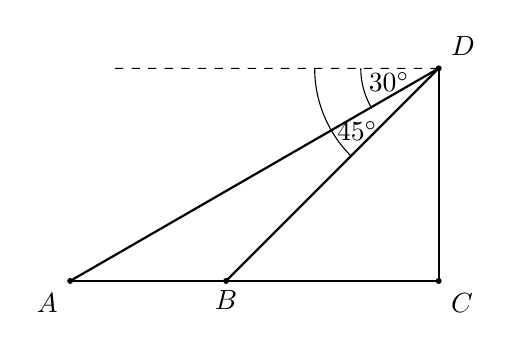
\begin{tikzpicture}[scale=0.9, line join=round]
  \coordinate (A) at (-5.2,0);
  \coordinate (B) at (-3,0);
  \coordinate (C) at (0,0);
  \coordinate (D) at (0,3);
  \draw[thick] (A) -- (C);
  \draw[thick] (C) -- (D);
  \draw[thick] (D) -- (A);
  \draw[thick] (D) -- (B);
  \draw[dashed] (D) -- (-4.6,3);
  \fill (A) circle (1.2pt) node[below left=1pt] {$A$};
  \fill (B) circle (1.2pt) node[below] {$B$};
  \fill (C) circle (1.2pt) node[below right=1pt] {$C$};
  \fill (D) circle (1.2pt) node[above right=1pt] {$D$};
  \draw (-1.1,3) arc[start angle=180, end angle=210, radius=1.1];
  \draw (-1.75,3) arc[start angle=180, end angle=225, radius=1.75];
  \node at (-0.70,2.81) {$30^\circ$};
  \node at (-1.15,2.12) {$45^\circ$};
\end{tikzpicture}
\end{center}
\nopagebreak[4]
\Needspace{4\baselineskip}
\textbf{解析}
\nopagebreak[4]
\begin{center}% 1977 年安徽卷（文科）第 8 题：山顶 D 测山高示意图（按源卷布局）
% DC 垂直于基线 AC（直角在 C，原图未画直角标记），过 D 水平虚线；
% 俯角 30° 弧（水平线到 DA）与 45° 弧（水平线到 DB）标在 D 处，
% 45° 标签按原图写在视线 DA 与 DB 之间。
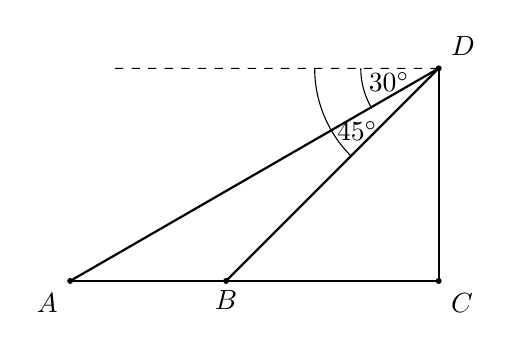
\begin{tikzpicture}[scale=0.9, line join=round]
  \coordinate (A) at (-5.2,0);
  \coordinate (B) at (-3,0);
  \coordinate (C) at (0,0);
  \coordinate (D) at (0,3);
  \draw[thick] (A) -- (C);
  \draw[thick] (C) -- (D);
  \draw[thick] (D) -- (A);
  \draw[thick] (D) -- (B);
  \draw[dashed] (D) -- (-4.6,3);
  \fill (A) circle (1.2pt) node[below left=1pt] {$A$};
  \fill (B) circle (1.2pt) node[below] {$B$};
  \fill (C) circle (1.2pt) node[below right=1pt] {$C$};
  \fill (D) circle (1.2pt) node[above right=1pt] {$D$};
  \draw (-1.1,3) arc[start angle=180, end angle=210, radius=1.1];
  \draw (-1.75,3) arc[start angle=180, end angle=225, radius=1.75];
  \node at (-0.70,2.81) {$30^\circ$};
  \node at (-1.15,2.12) {$45^\circ$};
\end{tikzpicture}
\end{center}
\nopagebreak[4]
\Needspace{5\baselineskip}
过 $D$ 的水平线与视线 $DA\text{、}DB$ 的夹角即俯角，且 $DC\perp AC$，故

\nopagebreak[4]
\[
\angle DAC=30^\circ,
\qquad
\angle DBC=45^\circ.
\]

\Needspace{5\baselineskip}
在直角三角形 $\triangle ACD$ 与 $\triangle BCD$ 中分别有

\nopagebreak[4]
\[
AC=CD\cot30^\circ,
\qquad
BC=CD\cot45^\circ=CD.
\]

\Needspace{5\baselineskip}
由 $AC-BC=AB=40$ 得

\nopagebreak[4]
\[
CD(\cot30^\circ-\cot45^\circ)=CD(\sqrt3-1)=40,
\]

\nopagebreak[4]
\[
CD=\frac{40}{\sqrt3-1}=\frac{40(\sqrt3+1)}{2}=20(\sqrt3+1)\approx54.6\ \text{\text{米}}.
\]

\begin{gktip}
\textbf{源注}：源解答答句印作「答：山高约55米」，与题面「精确到 0.1」的精度要求不符，本库按 $20(\sqrt3+1)\approx54.6$ 米作答；源解答中间一行还把该等式末尾排印作「$40$」后带度数符号（衍字）。源解答另给出利用 $AD=2CD$ 布列二次方程 $CD^2-40\,CD-800=0$ 的方法，结论相同。
\end{gktip}

\gkanswer{答案：山高 $CD=20(\sqrt3+1)\approx54.6$ 米。}

\end{answer}
\begin{answer}
\gksolhead{9}{}

\textbf{题目}（本题8分）：

红旗大队粮食产量逐年增加，1973年产量为90万斤，连续三年平均每年比前一年增产10\%，这个大队从1973年到1976年总共生产粮食多少万斤？（精确到0.1）

\Needspace{4\baselineskip}
\textbf{解析}

\Needspace{5\baselineskip}
1973 年至 1976 年共四个年度的产量组成等比数列，其中 $a_1=90$，公比 $q=1+10\%=1.1$，项数 $n=4$：

\nopagebreak[4]
\[
S_4=\frac{a_1(q^4-1)}{q-1}
=\frac{90\times(1.1^4-1)}{0.1}
=900\times(1.4641-1)=417.69\approx417.7\ \text{\text{万斤}}.
\]

（源注：源解答亦注明可先分别求各年产量再求和。）

\gkanswer{答案：约 $417.7$ 万斤。}

\end{answer}
\begin{answer}
\gksolhead{10}{}

\textbf{题目}（本题10分）：

求椭圆 $25x^2+9y^2=100$ 的长轴和短轴的长、焦点坐标，并且画出它的图象。

\Needspace{4\baselineskip}
\textbf{解析}

\Needspace{5\baselineskip}
方程两边同除以 $100$，化为标准形式：

\nopagebreak[4]
\[
\frac{x^2}{4}+\frac{y^2}{\frac{100}{9}}=1.
\]

\Needspace{5\baselineskip}
因为 $\dfrac{100}{9}>4$，椭圆的焦点在 $y$ 轴上，且

\nopagebreak[4]
\[
a=\frac{10}{3},
\qquad
b=2,
\qquad
c=\sqrt{a^2-b^2}=\sqrt{\frac{100}{9}-4}=\frac{8}{3}.
\]

\Needspace{5\baselineskip}
所以长轴长

\nopagebreak[4]
\[
2a=\frac{20}{3}=6\frac{2}{3},
\qquad
\text{\text{短轴长}}\ 2b=4,
\]

两个焦点坐标分别是 $\left(0,-2\frac{2}{3}\right)$ 和 $\left(0,2\frac{2}{3}\right)$。

图象：中心在原点、长轴在 $y$ 轴上的椭圆，四个顶点为 $(\pm2,0)$ 与 $\left(0,\pm\frac{10}{3}\right)$，过这四点用平滑曲线连成椭圆即得。

\gkanswer{答案：长轴长 $2a=\dfrac{20}{3}=6\frac{2}{3}$，短轴长 $2b=4$，焦点坐标 $(0,-2\frac{2}{3})$ 和 $(0,2\frac{2}{3})$；图象作法见解析版。}

\end{answer}